% !TEX root = ../../../Masterthesis.tex

\chapter{Star Trek II: The Wrath of Khan}

\section{Main Title}\label{sec:st 2 main title}
%-----------------------------------------------------------------------------
% Introduction
%-----------------------------------------------------------------------------
\begin{figure}[h!]
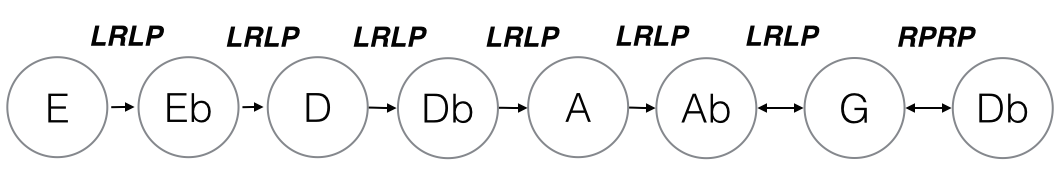
\includegraphics[width=\linewidth]{ST2_main_title_intro}
	\caption{ST 2: Main Title Introduction}
	\label{ST2_main_title_intro}
	\setfloatalignment{b}
\end{figure}
\noindent\newthought{A synth provides} a slowly evolving mysterious pad while the logos pass the screen. Soon after, we are traveling slowly through space and the trumpets play the Star Trek theme sequenced chromatically, figure \ref{ST2_main_title_intro}, from E downward to \eflat. The horns start playing a fiery sextuplet pattern in D doing a sort of call-and-response with the trumpets, sequencing downwards chromatically one more step to \dflat. Horner now repeats the sextuplet theme once more, but does a mediant modulation to A; the combined melodies create a whole tone feeling [1,3,5,9,E]\footnote{\keyboard{Ciss,Diss,F,A,B}}. On m.12, the Star Trek Logo is seen moving into screen and it conforms to the screen by m.13. The tonal center in \textbf{m.}11-12 is G, flanked by a predominant chord substitute, \aflat and a \acf{MTTP} to \dflat.



%-----------------------------------------------------------------------------
% A
%-----------------------------------------------------------------------------
\begin{figure}[h!]
\center
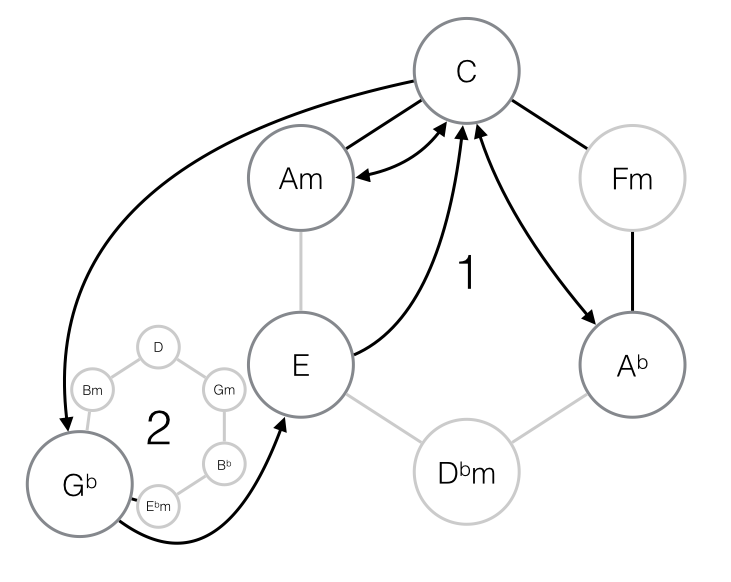
\includegraphics[width=0.7\linewidth]{ST2_main_title_a_pass_1}
	\caption{ST 2: Main Title A, pass 1}
	\label{ST2_main_title_a_pass_1}
	\setfloatalignment{b}
\end{figure}

The main theme is fanfare in C, figure \ref{ST2_main_title_a_pass_1}, but as one might expect from James Horner, the tonality is based on different circle then that of fifths. Instead of maneuvering in \textbf{NR\(_{1}\)}, he makes a short detour to \textbf{NR\(_{2}\)} to fetch \gflat. The melody uses the fifth mode of the melodic minor scale, i.e. the so called mixolydian \(\flatx{6}\) [0,2,4,5,7,8,T]\footnote{\keyboard{C,D,E,F,G,Giss,Aiss}}. A duality might be assumed by the fact that both Ionian, with the occurrence of [9], and melodic minor [8,10] is explored within the same phrase. 

\begin{figure}[h!]
\center
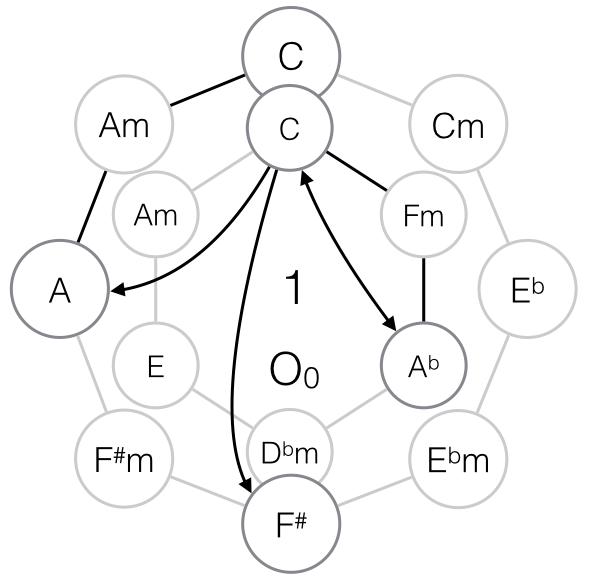
\includegraphics[width=0.7\linewidth]{ST2_main_title_a_pass_2}
	\caption{ST 2: Main Title A, pass 2}
	\label{ST2_main_title_a_pass_2}
	\setfloatalignment{b}
\end{figure}

The second pass, figure \ref{ST2_main_title_a_pass_2} holds the same harmonic idea but uses A instead of Am, making the progression almost completely Octatonic.\footnote{Much like we find in Goldsmith's harmonic language.} 

%-----------------------------------------------------------------------------
% B and C
%-----------------------------------------------------------------------------
\begin{figure}[h!]
\center
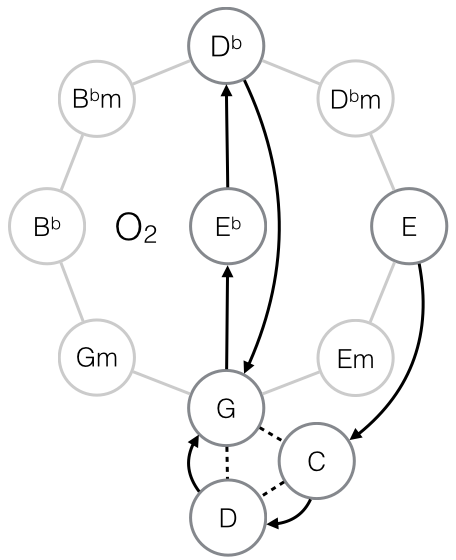
\includegraphics[width=0.7\linewidth]{ST2_main_title_b}
	\caption{ST 2: Main Title B}
	\label{ST2_main_title_b}
	\setfloatalignment{b}
\end{figure}

B starts with a triplet ostinato over E(\(\sharpx 5\)), played by the cellos, figure \ref{ST2_main_title_b}. The sense of Cartesian dualism intensifies with the continued mixolydian \(\flatx{6}\), cross combining major and minor. Harmonically the difference between A and B is enough to distinguish them, but the melody plays a variation on the main theme making the whole section somewhat familiar, yet distant to its origin. On bar 4 m.26, Horner starts a cascading flurry of chords, seemingly unrelated, but seen through \ac{nRT}, there is a clear idea driving the progression. From E, Horner makes a plagal cadence \(IV-V\) to G before moving through \(\flatx{VI}-\sharpx{IVb}\), making the bass line reminiscent of an Aeolian Cadence \(\flatx{VI}-\flatx{VII}-I\). m.32 lands on G while the melody is working a chromatically altered octatonic scale. 

%-----------------------------------------------------------------------------
% A and B'
%-----------------------------------------------------------------------------
\begin{figure}[h!]
\center
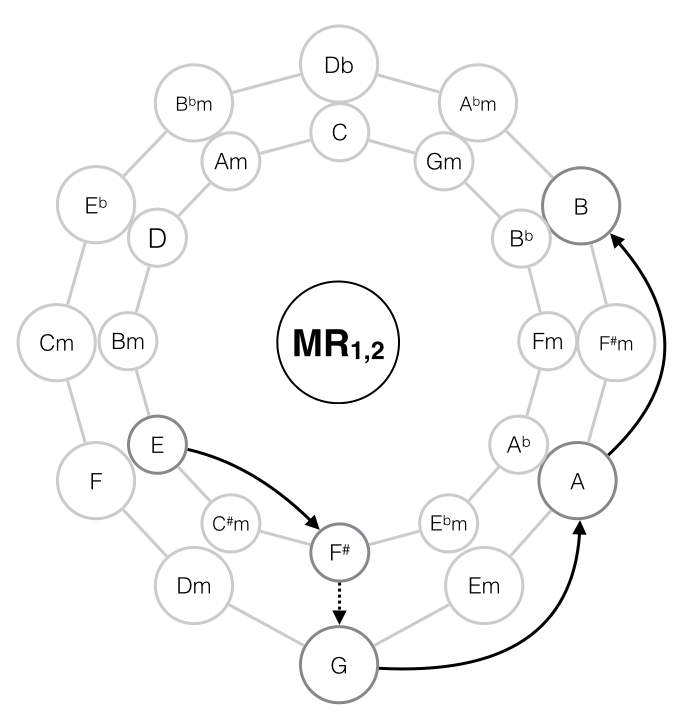
\includegraphics[width=0.7\linewidth]{ST2_main_title_b'}
	\caption{ST 2: Main Title B'}
	\label{ST2_main_title_b'}
	\setfloatalignment{b}
\end{figure}
After a reprise of A, a longer variation of B is developed, beginning at m.40, figure \ref{ST2_main_title_b'}. This time the low strings are playing melody while the high strings are playing the virtuositic sextuplet ostinato. This is the same ostinato that earlier was played as an arpeggiated \chord{E}{aug}, only double time. The harmonic backdrop moves through the \textbf{MR} circles, making a network modulation when jumping from \fiss to G. The melody follows the harmonic structure until m.48 where it follows the phrygian dominant scale [0,1,4,5,7,8,T]. The part repeats with the melody  played by the high strings, ever so slightly altered, and the ostinato returns to the previous pattern.

%-----------------------------------------------------------------------------
% Ending
%-----------------------------------------------------------------------------
The ending introduces itself in m.56, figure \ref{ST2_main_title_ending}, where Courage's Star Trek theme rings in with a lone trumpet. All the while, the strings play the same  phrygian dominant scale as a counterpoint, landing on B. From there the fanfare theme is used, sequencing ever upwards. If one were to see the final C as Tonic, the progression would follow: \(III-(MTTP)-\flatx{VII}-(Mediant)-II-\flatx{II}-(tritone substitute)-I\), making it a heavily distorted \(iii-vi-ii-V-I\). 

\clearpage
\begin{figure}
\center
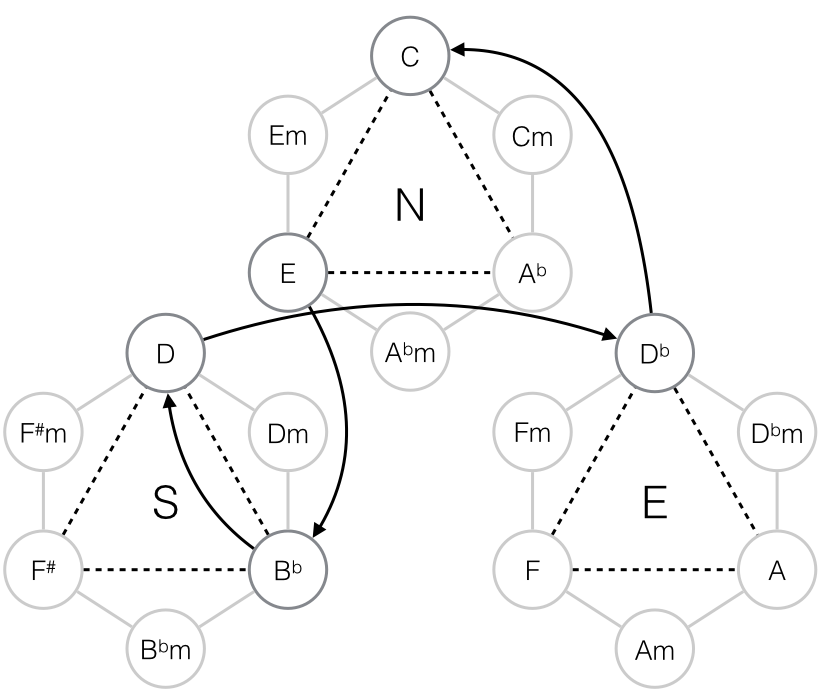
\includegraphics[width=\linewidth]{ST2_main_title_ending}
	\caption{ST 2: Main Title Ending}
	\label{ST2_main_title_ending}
	%\setfloatalignment{b}
\end{figure}



%-----------------------------------------------------------------------------
% PDF
%-----------------------------------------------------------------------------
\clearpage
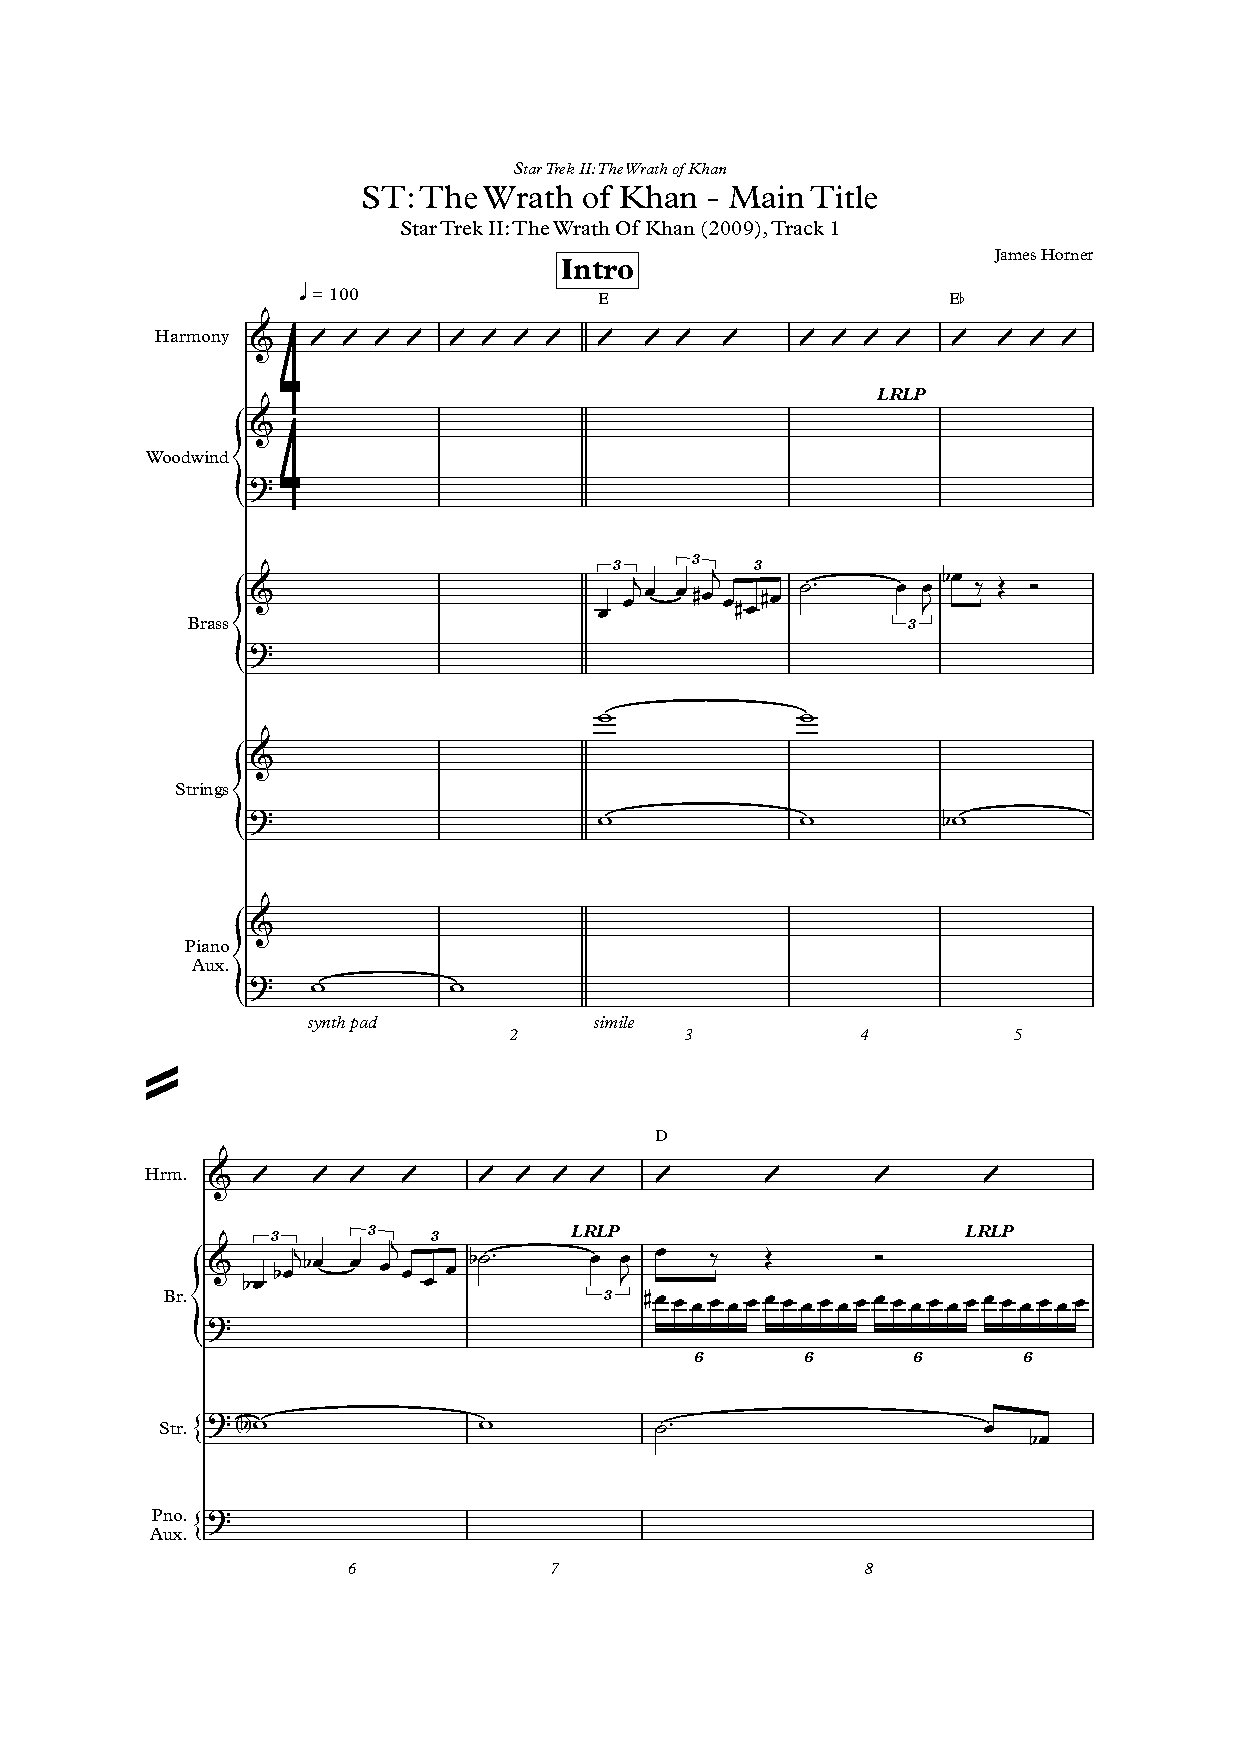
\includepdf[pages=-,pagecommand=\thispagestyle{fancy}]{pdf/ST2/ST2_Main_Title}

% Reviewed